%%%%%%%%%%%%%%%%%%%%%%%%%%%%%%%%%%%%%%%%%
% Thin Sectioned Essay
% LaTeX Template
% Version 1.0 (3/8/13)
%
% This template has been downloaded from:
% http://www.LaTeXTemplates.com
%
% Original Author:
% Nicolas Diaz (nsdiaz@uc.cl) with extensive modifications by:
% Vel (vel@latextemplates.com)
%
% License:
% CC BY-NC-SA 3.0 (http://creativecommons.org/licenses/by-nc-sa/3.0/)
%
%%%%%%%%%%%%%%%%%%%%%%%%%%%%%%%%%%%%%%%%%

%----------------------------------------------------------------------------------------
%    PACKAGES AND OTHER DOCUMENT CONFIGURATIONS
%----------------------------------------------------------------------------------------

\documentclass[a4paper, 11pt]{article} % Font size (can be 10pt, 11pt or 12pt) and paper size (remove a4paper for US letter paper)

\usepackage[protrusion=true,expansion=true]{microtype} % Better typography
\usepackage{graphicx} % Required for including pictures
\usepackage{wrapfig} % Allows in-line images
\usepackage{amsmath}
\usepackage{amsbsy}
\usepackage{amsthm}
\usepackage{amssymb}
\usepackage{mathpazo} % Use the Palatino font
\usepackage[T1]{fontenc} % Required for accented characters
\linespread{1.05} % Change line spacing here, Palatino benefits from a slight increase by default
\newcommand{\LL}{\mathcal{L}}
\newcommand{\q}{\tilde{q}}
\newcommand{\x}{\tilde{x}}
\newtheorem{Lemma}{Lemma}
\newtheorem{Theorem}{Theorem}
%\makeatletter
%\renewcommand\@biblabel[1]{\textbf{#1.}} % Change the square brackets for each bibliography item from '[1]' to '1.'
%\renewcommand{\@listI}{\itemsep=0pt} % Reduce the space between items in the itemize and enumerate environments and the bibliography
%
%\renewcommand{\maketitle}{ % Customize the title - do not edit title and author name here, see the TITLE block below
%\begin{flushright} % Right align
%{\LARGE\@title} % Increase the font size of the title
%
%\vspace{50pt} % Some vertical space between the title and author name
%
%{\large\@author} % Author name
%\\\@date % Date
%
%\vspace{40pt} % Some vertical space between the author block and abstract
%\end{flushright}
%}

%----------------------------------------------------------------------------------------
%    TITLE
%----------------------------------------------------------------------------------------

%\title{\textbf{Unnecessarily Long Essay Title}\\ % Title
%Focused and Deliciously Witty Subtitle} % Subtitle
%
%\author{\textsc{Ford Prefect} % Author
%\\{\textit{Interstellar University}}} % Institution
%
%\date{\today} % Date

%----------------------------------------------------------------------------------------

\begin{document}

%\maketitle % Print the title section

%----------------------------------------------------------------------------------------
%    ABSTRACT AND KEYWORDS
%----------------------------------------------------------------------------------------

%\renewcommand{\abstractname}{Summary} % Uncomment to change the name of the abstract to something else

%\begin{abstract}
%
%\end{abstract}
%
%\hspace*{3,6mm}\textit{Keywords:} lorem , ipsum , dolor , sit amet , lectus % Keywords
%
%\vspace{30pt} % Some vertical space between the abstract and first section

%----------------------------------------------------------------------------------------
%    ESSAY BODY
%----------------------------------------------------------------------------------------

\section{Introduction}
Valuing storage is a problem of significant interest in recent years, especially for energy-related commodities. Without storage, in an environment with either relatively stable supply and fluctuating demand, or relatively stable demand and fluctuating supply, prices vary significantly over time. This price variation generates an incentive to shift supply from a period where it is in excess, to a period where it is in shortage. Storage derives its economic value from exploiting these predictable price fluctuations by shifting supply over time.

Overview of storage valuation literature.

In this paper, we study the problem of valuing storage specifically for the case of energy commodities. We can develop a semi-analytical framework to price storage, allowing for mean-reverting price dynamics for the commodity, and general injection and withdrawal costs. Our framework is a generalization of the moving boundary method, described in \cite{}.

Overview of moving boundary method.

We apply our framework to study the value and optimal injection and withdrawal strategies for a calibrated example of crude oil/natural gas storage facility.


\section{Model}

Let $S_t$ be the price and its evolution follows 
\begin{equation}
  dS_t = \kappa(\gamma-\log(S_t))S_t dt + \sigma S_t dZ_t.
\end{equation}

Take $X_t = \log(S_t)$, by Ito's formula,
\begin{equation}
  dX_t = \kappa(\alpha - X_t) dt + \sigma dZ_t,
\end{equation}

where $\alpha = \gamma - \frac{\sigma^2}{2\kappa}$.\\ 

Denote the total amount of the commodity in the storage facility at time $t$ as $Q_t$. Also, denote cumulative amounts of the commodity purchased and sold up to time $t$ as $L_t$ and $U_t$, respectively. Here and after, buy and injection have the same meaning, so do sell and withdrawal. By definition, $L_t$ and $U_t$ are non-negative monotone cadlag processes, and 
    \begin{equation}\label{Eq:QLU}
    \begin{split}
      Q_t = Q_0 + L_t - U_t.
    \end{split}
    \end{equation}
Implied by (\ref{Eq:QLU}), $Q_t$ is of bounded variation.

The decisions are when and how much shall be injected and withdrawn from the facility. In other words, every decision can be represented as a pair $(L_t,U_t)$. An admissible control policy $(L_t,U_t)$ must satisfy that the storage level at any time is within capabilities. That is to say, $Q_t \in [Q_{\min},Q_{\max}]$ for all $t$ where $Q_{\min}$ and $Q_{\max}$ are the upper and lower capability respectively. We use $\mathcal{U}$ to denote all admissible policies.\\
%Because the change in storage is equal to the amount injected minus the amount withdrawn, we have
%\begin{equation}
%  dQ_t = dL_t - dU_t.
%\end{equation}

Both injection and withdrawal generate costs. As a result, injection and withdrawal won't take place at the same time. Let $\lambda(q)$ and $\mu(q)$ be the instantaneous costs of injection and withdrawal when the storage has $q$ units. Therefore, the costs of injection and withdrawal at time $t$ should be $\int_{Q_{t-}}^{Q_{t}} \lambda(q) dq$ and $\int_{Q_{t}}^{Q_{t-}} \mu(q) dq$ respectfully.

%todo: This part may not be necessary.
It is often easier to inject (withdraw) when empty (full) than full (empty). Therefore, we assume that $\lambda(q)$ is increasing with respect to $q$ while $\mu(q)$ is decreasing. To be economic meaningful, we also assume that $\lambda(q)$ and $\mu(q)$ are bounded.\\

We define the discounted infinite-horizon cash flows w.r.t. an admissible control policy $(L_t,U_t)$ as
\begin{equation}\label{Eq:V_LU}
\begin{split}
  V_{(L_t,U_t)}(x,q) = \mathbb{E}_{x,q} \left(\int_{0}^{\infty} e^{-\beta t}(e^{X_t} - M_t)dU_t - \int_{0}^{\infty}e^{-\beta t}(e^{X_t} + \Lambda_t)dL_t\right).
\end{split}
\end{equation}
Here $X_0 =x$, $Q_0 = q$, and discount factor $\beta \in (0,1)$. We use $\Lambda_t$ and $M_t$ to represent the injection and withdrawal cost at time $t$. By the definition of $\lambda$ and $\mu$, we have the following relations.
\begin{equation}
  \Lambda_t = \left\{
  \begin{array}{lc}
  \lambda(Q_t) & \mbox{if} ~ \Delta L_t = 0\\
  \frac{1}{\Delta L_t}\int_{Q_{t-}}^{Q_{t-} + \Delta L_t} \lambda(q) dq & \mbox{otherwise.}
  \end{array}
  \right.
\end{equation}
\begin{equation}
  M_t = \left\{
  \begin{array}{lc}
  \mu(Q_t) & \mbox{if} ~ \Delta U_t = 0\\
  \frac{1}{\Delta U_t}\int_{Q_{t-}-\Delta U_t}^{Q_{t-}} \mu(q) dq & \mbox{otherwise.}
  \end{array}
  \right.
\end{equation}

The objective is to choose the best $(L_t,U_t)$ that maximize the discounted infinite-horizon cash flows, 
\begin{equation}\label{Eq:V(x,q)}
  V(x,q) = \max_{(L,U) \in \mathcal{U}} V_{(L_t,Q_t)}(x,q).
\end{equation}

In other words, the maximum value that a facility manager can obtain from a storage facility when the current spot log price is $x$ and the amount is $q$ is $V(x,q)$. We call $V(x,q)$ the (optimal) value function and $V_{(L_t,U_t)}(x,q)$ the value function w.r.t strategy $(L_t,U_t)$.

\section{HJB equation, Verification Theorem, and the Choice of Search Space}
\subsection{HJB equation}

Bellman's principle of optimality together with It\^o's formula are commonly used to develop the necessary conditions of the optimal value function. Those necessary conditions are often called Hamilton-Jacobi-Bellman (HJB) equations.

%todo: Rewrite the following paragraph because it is copied from Haoling's paper.

The intuition behind the Bellman's principle of optimality is that if at time zero we use an arbitrary control for an infinitesimal amount of time, and immediately switch to the optimal control, then the resulting value function cannot be larger than the optimal one. Suppose for now that an optimal control exists, and denote it by $(L^*_t,U^*_t)$. Then, if we choose not to act during $t\in [0,\Delta t)$, for some small $\Delta t>0$ and then switch to the optimal policy $(L^*_t,U^*_t)$ thereafter, we will have

\begin{equation*}
\begin{split}
  V(x,q) &\geq \mathbb{E}_x\left(\int_{\Delta t}^{\infty} e^{-\beta t}(e^{X_t} - M_t)dU_t - \int_{\Delta t}^{\infty}e^{-\beta t}(e^{X_t} + \Lambda_t)dL_t\right) \\
  &= \mathbb{E}_x\left(e^{-\beta \Delta t} V(X_{\Delta t},q)\right)
\end{split}
\end{equation*}

Letting $\Delta t \rightarrow 0$, assuming sufficient smoothness of $V(\cdot,\cdot)$ and applying It\^{o}'s formula, we have
\begin{equation*}
\begin{split}
  \frac{1}{2}\sigma^2V_{xx}(x,q) + k(\alpha-x)V_{x}(x,q) - \beta V(x,q) \leq 0
\end{split}
\end{equation*}
Where $V_{x}$ ($V_{q}$) denotes the partial differential of $V$ with respect to $x$ ($q$), and $V_{xx}$ represents $\frac{\partial^2 V}{(\partial x)^2}$.


Next, say we choose to withdraw a small amount, $\Delta q$, instantaneously  and follow the optimal policy $(\hat{L}_t,\hat{U}_t)$ after that, we will have
\begin{equation*}
\begin{split}
  V(x,q) \geq V(x,q-\Delta q) + \int_{q}^{q+\Delta q}(e^x - \mu(l))dl.
\end{split}
\end{equation*}
Taking $\Delta q \rightarrow 0$, we have
\begin{equation*}
\begin{split}
  - V_q(x,q) + (e^x - \mu(q)) \leq 0.
\end{split}
\end{equation*}
Similarly, we can choose to instantaneously inject, and follow above arguments to have
\begin{equation*}
\begin{split}
  V_q(x,q) - (e^x - \lambda(q)) \leq 0.
\end{split}
\end{equation*}

Introduce the following three operators,
\begin{equation}\label{Oper}
\begin{split}
  \mathcal{L}V(x,q) &= \frac{1}{2}\sigma^2V_{xx}(x,q) + k(\alpha-x)V_{x}(x,q) - \beta V(x,q),\\
  \mathcal{S}V(x,q) &= -V_q(x,q) + (e^x - \mu(q)),\\
  \mathcal{B}V(x,q) &= V_q(x,q) - (e^x - \lambda(q)).
\end{split}
\end{equation}


Intuitively one of the three actions (holding, withdrawal and injection) should be optimal. Thus the value function $V(x,q)$ is expected to satisfy the HJB equation
\begin{equation}\label{HJB}
  \max \left[ \mathcal{L} V(x,q),\mathcal{S}V(x,q),\mathcal{B}V(x,q)\right] = 0.
\end{equation}


Because the three terms in equation (\ref{HJB}) are the profits utilizing holding, selling, and buying policy respectively,  they are called holding, selling, and buying profit.\\

In the next section, we will prove that HJB equation is sufficient as long as certain conditions are satisfied.

\subsection{Verification Theorem}

\begin{Theorem}
    Suppose $f(x,q) \in C^{2,1}(\mathbb{R} \times \mathbb{R})$ and both $f$ and $f_x$ are bounded. If $f$ satisfies 
    \begin{equation}\label{Eq:3max<=0}
    \begin{split}
        \max\left(\mathcal{L}f,\mathcal{B}f,\mathcal{S}f\right)(x,q) = 0,\quad (x,q)\in\mathbb{R}^2    ,
    \end{split}
    \end{equation}
    we have
    \begin{equation*}
    \begin{split}
        f(x,q) = V(x,q),
    \end{split}
    \end{equation*}
    where $V(x,q)$ is defined in (\ref{Eq:V(x,q)}).
\end{Theorem}

\begin{proof}
Because of (\ref{Eq:QLU}) and the monotonicity of processes $L_t$ and $U_t$, $Q_t$ is of finite variation. Combined with the assumption that $f \in C^{2,1}(\mathbb{R}\times \mathbb{R})$, we are able to use Ito's formula from (Protter 2005) to have
\begin{equation*}
\begin{split}
    e^{-\beta t} f(X_t,Q_t) - f(x,q) &= \int_{0}^t e^{-\beta s} \mathcal{L}f(X_s,Q_{s-})ds + \int_{0}^t e^{-\beta s} f_x(X_s,Q_{s-})dW_s \\
    &+ \int_{0}^{t} e^{-\beta s} f_q(X_s,Q_{s-}) dQ_s^c + \sum_{0\leq s\leq t}\left(e^{-\beta s} f(X_s,Q_s) - e^{-\beta s} f(X_s,Q_{s-})\right),  
\end{split}
\end{equation*}
where $X_0 = x$, $Q_{0-} = q$ and $Q_{\cdot}^c$ is the continuous part of $Q_{\cdot}$. This equation is valid for arbitrary $Q_t$ that satisfies (\ref{Eq:QLU}). Because both $f$ and $f_x$ are bounded, we can take expectation to both sides and then take $t \rightarrow \infty$,
\begin{equation*}
\begin{split}
  f(x,q) = &- \mathbb{E}\int_{0}^{\infty}e^{-\beta t}\mathcal{L}f(X_t,Q_{t-}) dt - \mathbb{E}\int_{0}^{\infty}e^{-\beta t}f_q(X_t,Q_{t-})dQ_t^c \\
  & - \mathbb{E} \sum_{0\leq t <\infty}\left(e^{-\beta t} f(X_t,Q_t) - e^{-\beta s} f(X_t,Q_{t-})\right).
\end{split}
\end{equation*}
Plug (\ref{Eq:QLU}) into,
\begin{equation}\label{Eq:Ito}
\begin{split}
  f(x,q)  &=  - \mathbb{E}\int_{0}^{\infty}e^{-\beta t}\mathcal{L}f(X_t,Q_{t-}) dt \\
  & \quad - \mathbb{E}\int_{0}^{\infty}e^{-\beta t}f_q(X_t,Q_{t-})dL_t^c + \mathbb{E}\int_{0}^{\infty}e^{-\beta t}f_q(X_t,Q_{t-})dU_t^c \\
  & \quad - \mathbb{E} \sum_{0\leq t <\infty}\left(e^{-\beta t} f(X_t,Q_{t-}+\Delta L_t) - e^{-\beta t} f(X_t,Q_{t-})\right) \\
  & \quad - \mathbb{E} \sum_{0\leq t <\infty}\left(e^{-\beta t} f(X_t,Q_{t-}-\Delta U_t) - e^{-\beta t} f(X_t,Q_{t-})\right)\\
  & = - \mathbb{E}\int_{0}^{\infty}e^{-\beta t}\mathcal{L}f(X_t,Q_{t-}) dt \\
  & \quad - \mathbb{E}\int_{0}^{\infty}e^{-\beta t}f_q(X_t,Q_{t-})dL_t^c + \mathbb{E}\int_{0}^{\infty}e^{-\beta t}f_q(X_t,Q_{t-})dU_t^c \\
  & \quad - \mathbb{E} \sum_{0\leq t <\infty}\left(e^{-\beta t} \int_{Q_{t-}}^{Q_{t-}+\Delta L_t} f_q(X_t,q) dq\right) \\
  & \quad + \mathbb{E} \sum_{0\leq t <\infty}\left(e^{-\beta t} \int_{Q_{t-}-\Delta U_t}^{Q_{t-}}f_q(X_t,q)dq \right).\\
\end{split}
\end{equation}
From (\ref{Eq:3max<=0}), we have $\mathcal{L}f(x,q) \leq 0$ and $e^x -\mu(q)\leq  f_q(x,q)\leq e^x + \lambda(q)$ hold for all $(x,q) \in \mathbb{R}^2$. Substitute them into (\ref{Eq:Ito}) to have
\begin{equation}\label{Eq:f>=V}
\begin{split}
  f(x,q) & \geq - \mathbb{E}\int_{0}^{\infty}e^{-\beta t}(e^{X_t} + \lambda(Q_{t-}))dL_t^c + \mathbb{E}\int_{0}^{\infty}e^{-\beta t}(e^{X_t} -\mu(Q_{t-}))dU_t^c \\
  & \quad - \mathbb{E} \sum_{0\leq t <\infty}\left(e^{-\beta t} \int_{Q_{t-}}^{Q_{t-}+\Delta L_t}(e^x + \lambda(q))  dq\right) \\
  & \quad + \mathbb{E} \sum_{0\leq t <\infty}\left(e^{-\beta t} \int_{Q_{t-}-\Delta U_t}^{Q_{t-}}(e^x - \mu(q))dq \right)\\
  & = \mathbb{E}_{x,q} \left(\int_{0}^{\infty} e^{-\beta t}(e^{X_t} - M_t)dU_t - \int_{0}^{\infty}e^{-\beta t}(e^{X_t} + \Lambda_t)dL_t\right).
\end{split}
\end{equation}
Because this inequality is true for all admissible $(L_t,U_t)$, by definition of $V(x,q)$, namely (\ref{Eq:V(x,q)}), we have 
\begin{equation*}
\begin{split}
  f(x,q) \geq V(x,q).
\end{split}
\end{equation*}
The region where the holding profit is the highest is called the optimal holding region and denoted as $H^*$. Similarly, the optimal selling (buying) region is defined and denoted as $S^*$ ($B^*$). Mathematically speaking, 
\begin{equation*}
\begin{split}
  \mathcal{L} V(x,q) &= \max \left[ \mathcal{L} V(x,q),\mathcal{S}V(x,q),\mathcal{B}V(x,q)\right] = 0 \quad (x,q) \in H^*\\
  \mathcal{S}V(x,q) &=\max \left[ \mathcal{L} V(x,q),,\mathcal{S}V(x,q),\mathcal{B}V(x,q)\right] = 0 \quad (x,q) \in S^*\\
  \mathcal{B}V(x,q) &=\max \left[ \mathcal{L} V(x,q),,\mathcal{S}V(x,q),\mathcal{B}V(x,q)\right] = 0 \quad (x,q) \in B^*.
\end{split}
\end{equation*}

Notice that the equality holds in (\ref{Eq:f>=V}) if 
\begin{equation*}
\begin{split}
  &\mathcal{L}f(X_t,Q_{t-}) = 0 \quad \forall t>0\\
  &\mathcal{S}f(X_t,Q_{t-}) = 0 \quad \mbox{if} ~ dU_t^c \neq 0~ \mbox{or}~ \Delta U_t \neq 0\\
  &\mathcal{B}f(X_t,Q_{t-}) = 0 \quad \mbox{if} ~ dL_t^c \neq 0~ \mbox{or}~\Delta L_t \neq 0\\  
\end{split}
\end{equation*}
Such admissible control $(L^*_t,U^*_t)$ can be found if we follow the rules that hold in $H^*$, sell in $S^*$, and buy in $B^*$. Thus, by definition of V(x,q),
\begin{equation*}
\begin{split}
  f(x,q) = V_{(L^*,U^*)}(x,q) \leq V(x,q).
\end{split}
\end{equation*}

\end{proof}

It is worth notice that the optimal policy $(L^*_t,U^*_t)$ is totally determined by the region triplet $(H^*,S^*,B^*)$. As a result, instead of searching $(L^*_t,U^*_t)$, we choose to search the region triplet $(H^*,S^*,B^*)$. This narrows down the policy space that we will search.

\subsection{Search Space}
If $\mathbb{R}^2$ is divided into holding region, H, selling region, S, and buying region, B, we can derive a related strategy $(L_t,U_t)$ following the rules that sell in S, buy in B, and hold in H. We call $(H,S,B)$ a region triplet and we also use it to represent related strategy.

\begin{Theorem}\label{Th:fix}
Let $v$ be the solution to
\begin{equation*}
\begin{split}
  & \mathcal{L} v = 0 \quad (x,q) \in H\\
  & \mathcal{S} v = 0 \quad (x,q) \in S\\
  & \mathcal{B} v = 0 \quad (x,q) \in B,
\end{split}
\end{equation*}
where $(H,S,B)$ is a region triplet. If $v \in C^{2,1}(\mathbb{R}\times\mathbb{R}/\partial H)$ and both $v$ and $v_x$ are bounded, $v$ is the value function w.r.t $(H,S,B)$.
\end{Theorem}

\begin{proof}
Let $(L_t,U_t)$ be the respective strategy w.r.t $(H,S,B)$ and we have
\begin{equation*}
\begin{split}
    &(X_t,Q_{t-}) \in H \quad \forall t >0\\
    &(X_t,Q_{t-}) \in \partial B \Leftrightarrow dL_t^c \neq 0\\
    &(X_t,Q_{t-}) \in \partial S \Leftrightarrow dU_t^c \neq 0\\
    &(X_t,Q_{t-}) \in B^o \Leftrightarrow \Delta L_t \neq 0\\
    &(X_t,Q_{t-}) \in S^o \Leftrightarrow \Delta U_t \neq 0\\
\end{split}
\end{equation*}

By (\ref{Eq:Ito}), we have
\begin{equation*}
\begin{split}
  v(x,q) & = - \mathbb{E}\int_0^{\infty} e^{-\beta t}(e^x + \lambda(q)) dL_t^c +  \mathbb{E}\int_0^{\infty} e^{-\beta t}(e^x - \mu(q)) dU_t^c\\
  & \quad - \mathbb{E} \sum_{0\leq t<\infty} e^{-\beta t}\int_{Q_{t-}}^{Q_{t-} + \Delta L_t}(e^x + \lambda(q))dq +\mathbb{E} \sum_{0\leq t<\infty} e^{-\beta t}\int_{Q_{t-}}^{Q_{t-} + \Delta L_t}(e^x + \lambda(q))dq\\
  & = \mathbb{E}\int_0^{\infty}e^{-\beta t}(e^x - M(q))dU_t - \mathbb{E} \int_0^{\infty}e^{-\beta t}(e^x +\Lambda(q))dL_t = V_{(L_t,U_t)}(x,q)
\end{split}
\end{equation*}


\end{proof}
HJB equation is a free-boundary problem which is hard to solve. Instead of solving it directly, we want to have a sequence of region triplets, $(H^{n},S^{n},B^{n})$, to approach the optimal regiones $(H^*,S^*,B^*)$. The fixed boundary problem $(H^{n},S^{n},B^{n})$ is defined as a system of equations which states that holding (selling, buying) profit is 0 in $H^{n}$ ($S^{n}, B^{n}$). Mathematically speaking, 
\begin{equation}\label{Eq:Vn}
\begin{array}{ll}
\mathcal{L} V^{n}(x,q) = 0& (x,q) \in H^{n}\\
\mathcal{S}V^{n}(x,q) = 0 &(x,q) \in S^{n}\\
\mathcal{B}V^{n}(x,q) = 0 &(x,q) \in B^{n}.\\
\end{array}
\end{equation}
Here the solution to the fixed boundary problem is denoted as $V^{n}(x,q)$.

\section{Algorithm}
\begin{enumerate}
  \item Find a large enough number $M_0$ such that the optimal selling region contains the inititial selling region $S^0 =  \{(x,q)|x\geq M_0,~Q_{\min} <q \leq Q_{\max}\}$. Set holding region $H^0 = (S^0)^c$ and buying region $B^0 = \emptyset$.   
  \item  Keep doing the following steps until convergence.
  \begin{enumerate}
  \item Calculate the value function $V^{n}(x,q)$.
  \item If the maximal selling profit is positive, $max_{x}\mathcal{S}V^{n}(x,q)>0$, then set the selling region $S^{n+1} = \{(x,q)|x\geq x_s^{n+1}(q)\}$ where 
    \begin{equation*}
      x_s^{n+1}(q) = \arg\max_{x} \mathcal{S}V^{n}(x,q) 
    \end{equation*}
  \item If the maximal buying profit is positive, $max_{x}\mathcal{B}V^{n}(x,q)>0$, then set the buying region $B^{n+1} = \{(x,q)|x_l^{n+1}(q)\leq x\leq x_u^{n+1}(q)\}$. There are two possibilities.
  \begin{enumerate}
  \item Buying region is empty at iteration $n$.
      \begin{equation*}
      x_l^{n+1}(q) = x_u^{n+1}(q) =\arg \max_{x} \mathcal{B}V^{n}(x,q).
    \end{equation*}
  
  \item Buying region is not empty at iteration $n$. 
    \begin{equation*}
    \begin{split}
        x_u^{n+1}(q) &= \arg\max_{x\geq x_u^{n}(q)} \mathcal{B}V^{n+1}(x,q),\\
        x_l^{n+1}(q) &= \arg\max_{x\leq x_l^{n}(q)} \mathcal{B}V^{n+1}(x,q).
    \end{split}
    \end{equation*} 
  \end{enumerate}

  
  \item Set the holding region as $H^{n+1} = (S^{n+1} \cup B^{n+1})^c$.
  \item $n = n + 1$.
  \end{enumerate}
\end{enumerate}

To show this algorithm works, four things need to be proved.
\begin{enumerate}
  \item The existence of $M_0$.
  \item $V^{n}$ is monotone increasing.
  \item The boundaries can keep moving.
  \item The convergence function is optimal.
\end{enumerate}


\subsection{The existence of $M_0$}

\begin{Lemma}\label{LemmaExiM_0}%existence of M_0
For any positive storage level, $\q>0$, there exists a number $M_0(\q)$ such that region $\{(x,q)| x \geq M_0(\q), q = \q\}$ is contained by the optimal selling region $S^*$.
\end{Lemma}

\begin{proof}
First, in order to make money, for any buying price, there must be a higher selling price. As a result, the optimal buying region won't contain a region with infinite upper bound. Thus if lemma \ref{LemmaExiM_0} doesn't hold, it is the optimal holding region $H^*$ that the region $\{(x,\q)|x>M_0(\q)\}$ belongs to. In other words, for any log price $x$ larger than the number $M_0(\q)$, 
    \begin{equation}\label{Eq:Hold}
    \begin{split}
    \LL V(x,\q) &=  0\\
    \mathcal{S} V(x,\q) &\leq 0.\\
    \mathcal{B} V(x,\q) &\leq 0\\
    \end{split}
    \end{equation}
Define
\begin{equation}\label{h}
h(x) = -\mathcal{S}V(x,\q) = V_q(x,\q) - (e^x -\mu(\q)).
\end{equation}
Because $- \mathcal{S}V(x,q) = \mathcal{B}V(x,q) + (\lambda(q) + \mu(q))$, together with the last two inequalities of (\ref{Eq:Hold}), we have 
\begin{equation}\label{hin}
0\leq h(x) \leq \lambda(\q) + \mu(\q) \quad \forall x > M_0(\q).
\end{equation}
On the other hand, take derivative with respect to $q$ to both sides of first equality of (\ref{Eq:Hold}) and we have $\LL V_q(x,\q) =  0$. Substitute (\ref{h}) into it to have 
\begin{equation*}
\frac{1}{2}\sigma^2h''(x) + k(\alpha-x)h'(x) - \beta h(x) = - \frac{1}{2}\sigma^2 e^x + k (x- \alpha)e^x + \beta(e^x - \mu(\q)).
\end{equation*}
Divide both sides by $e^x$,
\begin{equation}\label{hPDE}
  \frac{1}{2}\sigma^2e^{-x}h''(x) + ke^{-x}(\alpha-x)h'(x) - \beta e^{-x}h(x) = - \frac{1}{2}\sigma^2+ k (x- \alpha) + \beta(1 - e^{-x}\mu(\q)).
\end{equation}
Because the buying cost, $\mu(\q)$, is bounded, the right-hand side of (\ref{hPDE}) goes to the positive infinity when $x$ approaches the positive infinity. Meanwhile, by (\ref{hin}), function $h(x)$ is bounded. Combine these two, when $x$ approaches the positive infinity, either 
\begin{enumerate}
  \item $e^{-x}h''(x)\rightarrow +\infty$ or 
  \item $e^{-x}(\alpha-x)h'(x) \rightarrow +\infty$.
\end{enumerate}
In first case, because $e^{-x}h''(x)$ approaches the positive infinity when $x$ approaches positive infinity, there must exist a number $t_1$ such that $h''(x)$ is positive for any $x$ larger than $t_1$. For any $t_2$ larger than $t_1$, by Fubini's theorem, we have
\begin{equation}\label{Fubini}
\begin{split}
h(t_2) - h(t_1) &= \int_{t_1}^{t_2}h'(t)dt = \int_{t_1}^{t_2}(\int_{t_1}^{t}h''(x)dx+h'(t_1))dt\\
&=  \int_{t_1}^{t_2}\int_{t_1}^{t}h''(x)dxdt +(t_2-t_1)h'(t_1)\\
&= \int_{t_1}^{t_2}\int_{x}^{t_2}h''(x)dtdx +(t_2-t_1)h'(t_1)\\
&= \int_{t_1}^{t_2}(t_2-x)h''(x)dx +(t_2-t_1)h'(t_1)\\
&\geq e^{t_1} \int_{t_1}^{t_2}(t_2-x)e^{-x}h''(x)dx + (t_2-t_1)h'(t_1) \\
& = e^{t_1} \int_{t_1}^{t_2}\left((t_2-x)e^{-x}h''(x) + e^{-t_1}h'(t_1) \right)dx.
\end{split}
\end{equation}
With $t_1$ fixed, when $t_2 \rightarrow +\infty$, the right hand side approaches positive infinity. This is a contradiction with $(\ref{hin})$.\\
In the second case, because $e^{-x}(\alpha-x)h'(x)$ approaches the positive infinity when $x$ approaches positive infinity, there must exist a number $t_1 > \alpha$ such that $(\alpha -x)h'(x)$ is positive for any $x$ larger than $t_1$. On the other hand, $e^x/(\alpha -x)$ is a decreasing function when $x$ is large enough. Without losing any generality, assume it is decreasing for all $x$ that is bigger than $t_1$. For any $t_2$ larger than $t_1$, we have
\begin{equation}
\begin{split}
h(t_2) - h(t_1) &= \int_{t_1}^{t_2} h'(t)dt \\
&= \int_{t_1}^{t_2} \frac{e^t}{\alpha-t} \frac{(\alpha-t)h'(t)}{e^t}dt\\
&\leq \frac{e^{t_1}}{\alpha-t_1} \int_{t_1}^{t_2}\frac{(\alpha-t)h'(t)}{e^t}dt.
\end{split}
\end{equation}
With $t_1$ fixed, when $t_2 \rightarrow +\infty$, the right hand side approaches negative infinity. This is also a contradiction with $(\ref{hin})$.\\
\end{proof}

Because we use the discretization method to solve the HJB equation (\ref{HJB}), only finite number of $M_0(\q)$ matter. The maximal of those is $M_0$. A proposed $M_0$ is large enough if it satisfies
\begin{equation*}
  \left(\mathcal{S}V(x,q)\right)_x|_{x = M_0} < 0 \quad \forall q \in (Q_{\min},Q_{\max}].
\end{equation*}

\subsection{$V^{n}$ is monotone increasing}

\begin{Theorem}\label{incrs}
The value function $V^{n+1}$ with the region triplet $(H^{n+1},S^{n+1},B^{n+1})$ is larger than the value function $V^{n}$ with the regions triplet $(H^n,S^n,B^n)$.
\end{Theorem}

\begin{proof}

By equation (\ref{Eq:Vn}) and the way the algorithm works, for $V^n$, we have
  
\begin{equation}\label{Vn}
\begin{array}{ll}
\LL V^{n}(x,q) = 0& (x,q) \in H^{n}\\
-V^{n}_q(x,q) + e^x - \mu(q) = 0 &(x,q) \in S^{n}\\
-V^{n}_q(x,q) + e^x - \mu(q) > 0 &(x,q) \in S^{n+1}/S^{n}\\
V^{n}_q(x,q) - e^x - \lambda(q) = 0 & (x,q) \in B^{n}\\
V^{n}_q(x,q) - e^x - \lambda(q) > 0 & (x,q) \in B^{n+1}/B^{n}.\\
\end{array}
\end{equation}
For $V^{n+1}$, we have
\begin{equation}\label{Vn+1}
\begin{array}{ll}
\LL V^{n+1}(x,q) = 0& (x,q) \in H^{n+1}\\
-V^{n+1}_q(x,q) + e^x - \mu(q) = 0 &(x,q) \in S^{n}\\
-V^{n+1}_q(x,q) + e^x - \mu(q) = 0 &(x,q) \in S^{n+1}/S^{n}\\
V^{n+1}_q(x,q) - e^x - \lambda(q) = 0 & (x,q) \in B^{n}\\
V^{n+1}_q(x,q) - e^x - \lambda(q) = 0 & (x,q) \in B^{n+1}/B^{n}.\\
\end{array}
\end{equation}

The algorithm guarantees the monotonicity of $H^n,~S^n$ and $B^n$, that is to say, $H^{n} \supset H^{n+1},~S^{n} \subset S^{n+1}$ and $B^{n} \subset B^{n+1}$. Introduce $\Delta V^{n+1}(x,q) = V^{n+1}(x,q) - V^{n}(x,q)$. From (\ref{Vn}) and (\ref{Vn+1}), we can deduce   
\begin{equation}\label{dV}
\begin{split}
\LL \Delta V^{n+1}(x,q) &= 0 \quad (x,q) \in H^{n+1}\\
\Delta V_q^{n+1}(x,q) &= 0 \quad (x,q) \in S^{n}\\
\Delta V_q^{n+1}(x,q) &> 0 \quad (x,q) \in S^{n+1}/S^{n}\\
\Delta V_q^{n+1}(x,q) &= 0 \quad (x,q) \in B^{n}\\
\Delta V_q^{n+1}(x,q) &< 0 \quad (x,q) \in B^{n+1}/B^{n}.\\
\end{split}  
\end{equation}

By Theorem (\ref{Th:fix}), $\Delta V^{n+1}$ is the value function w.r.t regions triplet $(H^n,S^n,B^n)$ and positive selling profit and negative buying cost \footnote{It means that one can increase the volume in the storage and make a profit at the same time.}. As a result, for every regions triplet, the value function is positive, namely $\Delta V^{n+1} > 0$.

\end{proof}

\subsection{The boundaries can keep moving}

From the algorithm, the boundaries can move if and only if the following theorem holds.

\begin{Lemma}\label{maxi1}
If $\mathcal{L}f(x) = 0,~l\leq x \leq u$ and $f(l) <0, f(u) >0$, $f(u)$ is the maximum and $f(l)$ is the minimum.
\end{Lemma}
\begin{proof}
Assume $u$ is not the maximum, then $f$ must achieve the maximum at an interior point, denoted as $x_M$. Thus $f(x_M)> f(u)>0$, $f'(x_M) =0$, and $f''(x_M) \leq 0$. By $\mathcal{L}f(x_M) = 0$, 
    \begin{equation*}
    \begin{split}
          &\frac{1}{2}\sigma^2f''(x_M) + \kappa(\alpha - x_M)f'(x_M) - \beta f(x_M) = 0\\
          \Rightarrow~& 0< \beta f(x_M) = \frac{1}{2}\sigma^2f''(x_M) + \kappa(\alpha - x_M)f'(x_M) \leq 0
    \end{split}
    \end{equation*}
Contradiction! We can use the similar argument to prove $f(l)$ is the minimum.
\end{proof}


\begin{Theorem}
Three inequalities below are true for all integer $n$ and storage level $q$.
\begin{equation*}
\begin{split}
\left(\mathcal{S}V(x,q)\right)_x|_{x = x_s^{n+1}(q)} & < 0\\
\left(\mathcal{B}V(x,q)\right)_x|_{x = x_u^{n+1}(q)} & > 0\\
\left(\mathcal{B}V(x,q)\right)_x|_{x = x_l^{n+1}(q)} & < 0\\
\end{split}
\end{equation*}
When $x_u^{n+1}(q)$ and $x_l^{n+1}(q)$ don't exist, we assume the last two inequalities are true automatically.

\end{Theorem}

\begin{proof} 
Introduce function $f(x) = \Delta V_q^{n+1}(x,q)$ with any fixed storage level $q$. 
Differentiate (\ref{dV})the first equation with respect to $q$, we have 
\begin{equation*}
\begin{split}
  \mathcal{L} f(x) = 0,\quad x_u^{n+1}(q) \leq x \leq x_s^{n+1}(q)
\end{split}
\end{equation*}

By Lemma (\ref{maxi1}), $f(x)$ achieves its maximum at point $x_s^{n+1}(q)$. Therefore $f'(x_s^{n+1}(q)) > 0$ or  $f'(x_s^{n+1}(q)) = 0$. If the latter is true, from $\LL f(x_s^{n+1}(q)) = 0$, we have $0<\beta f(x_s^{n+1}(q)) = \frac{1}{2}\sigma^2 f''(x_s^{n+1}(q))\leq 0$ which is a contradiction. As a result, we proved that $f'(x_s^{n+1}(q)) > 0$.
\begin{equation}\label{EqKeepMove}
\begin{split}
&(\Delta V_q^{n+1})_x(x_s^{n+1}(q),q) = f'(x_s^{n+1}(q)) > 0\\
\Rightarrow & (V_q^{n+1})_x(x_s^{n+1}(q),q) -(V_q^{n})_x(x_s^{n+1}(q),q) >0\\
\Rightarrow & (V_q^{n+1})_x(x_s^{n+1}(q),q) - e^{x_s^{n+1}(q)} > 0 \\
\Rightarrow & \left(V_q^{n+1}(x,q) - (e^{x}-\mu(q)\right)_x|_{x = x_s^{n+1}(q)} > 0 \\ 
\Rightarrow & \left(-V_q^{n+1}(x,q) + (e^{x}-\mu(q)\right)_x|_{x = x_s^{n+1}(q)} < 0.\\
\Rightarrow & \left(\mathcal{S}V(x,q)\right)_x|_{x = x_s^{n+1}(q)}  < 0
\end{split}
\end{equation}
On the other hand, $f(x)$ achieves the minimum at $x_u^{n+1}(q)$ and $x_l^{n+1}(q)$. Using similar arguments as $x_s^{n+1}(q)$ to have 
\begin{equation*}
\begin{split}
\left(\mathcal{B}V(x,q)\right)_x|_{x = x_u^{n+1}(q)} & > 0\\
\left(\mathcal{B}V(x,q)\right)_x|_{x = x_l^{n+1}(q)} & < 0\\
\end{split}
\end{equation*}
\end{proof}

\section{$\epsilon$-Optimality}


\begin{Theorem}
Suppose $f \in C^{2,1}(\mathbb{R} \times \mathbb{R})$ and both $f$ and $f_x$ are bounded. If $f$ satisfies that $\mathcal{L}f \leq \epsilon$, $\max(\mathcal{B}f,\mathcal{S}f) \leq 0$, then $f(x,q) \geq V(x,q) - \frac{\epsilon}{\beta}$
\end{Theorem}

\begin{proof}
Because $f \in C^{2,1}(\mathbb{R} \times \mathbb{R})$ and both $f$ and $f_x$ are bounded, (\ref{Eq:Ito}) is valid. Plug $\mathcal{L}f \leq \epsilon$, $\max(\mathcal{B}f,\mathcal{S}f) \leq 0$ into (\ref{Eq:Ito}) and we have
\begin{equation*}
\begin{split}
  f(x,q) &\geq -\mathbb{E} \int_{0}^{\infty}e^{-\beta t} \epsilon dt + \mathbb{E}\left(\int_{0}^{\infty} e^{-\beta t}(e^{X_t} - M_t)dU_t - \int_{0}^{\infty}e^{-\beta t}(e^{X_t} + \Lambda_t)dL_t\right)\\
  & = V_{(L,U)}(x,q) - \frac{\epsilon}{\beta}.
\end{split}
\end{equation*}
Because this inequality holds for any admissible strategy $(L,U)$, we have $f(x,q) \geq V(x,q) - \frac{\epsilon}{\beta}$.

\end{proof}

\begin{Theorem}
Suppose $f \in C^{2,1}(\mathbb{R} \times \mathbb{R})$ and both $f$ and $f_x$ are bounded. If $f$ satisfies that $\max(\mathcal{L}f,\mathcal{B}f,\mathcal{S}f) \leq \epsilon$, then ???.
\end{Theorem}

\begin{proof}
Because $f \in C^{2,1}(\mathbb{R} \times \mathbb{R})$ and both $f$ and $f_x$ are bounded, (\ref{Eq:Ito}) is valid. Plug $\mathcal{L}f \leq \epsilon$, $\max(\mathcal{B}f,\mathcal{S}f) \leq 0$ into (\ref{Eq:Ito}) and we have
\begin{equation*}
\begin{split}
  f(x,q) &\geq -\mathbb{E} \int_{0}^{\infty}e^{-\beta t} \epsilon dt + \mathbb{E}\left(\int_{0}^{\infty} e^{-\beta t}(e^{X_t} - M_t- \epsilon)dU_t - \int_{0}^{\infty}e^{-\beta t}(e^{X_t} + \Lambda_t + \epsilon)dL_t\right)\\
  & = V_{(L,U)}(x,q) - \frac{\epsilon}{\beta} - \epsilon \mathbb{E}\int_0^{\infty}e^{-\beta t}(dU_t + dL_t).
\end{split}
\end{equation*}

\end{proof}


%
%
%
%
%
%
%
%
%
%
%
%Since there are only two activities, buy and sell, the way of making a profit must be buy low and sell high. Actually, it is rigorously proved that the optimal policy must sell when price is high enough. However, the existence of transaction costs implies that the real buying price which includes injecting cost has a lower bound $\lambda(q)$. Therefore, the minimal selling price is $\lambda(q)+\mu(q)$. In this case, we may not buy at extremely low price because it takes a long time to go back to $\lambda(q)+\mu(q)$ level which means it may be impossible to make a profit resulting from discounting. This can be seen clearly when $\lambda(q)+\mu(q)$ is larger than the mean reverting level $\alpha$\footnote{Is there certain constraints guarantee the existence of lower bound of buying region?}. Here comes the difficulty of moving boundary method. \\
%
%\textbf{No suitable initial guess for buying region exists. A initial guess needs to generated in the moving boundary method itself.}\\
%
%What will the optimal strategy be without buying? It will be less aggressive because there is only one chance for selling. In other words, the selling price will be higher. On the other hand, the probability a buying strategy makes money depends on the selling strategy. The better selling strategy the larger probability certain buying strategy will make a profit. If a buying strategy can make money with the optimal selling strategy without buying, it must be able to make money with the optimal one with buying. Actually, the optimal selling strategy without buying is not necessary. All we need is a selling strategy that is less aggressive than the global optimal.\\
%
%Here comes the method that overcome above difficulty.
%
%\begin{enumerate}
%  \item Assume there is no buying region at all while the selling strategy is selling all in stock at a super high price.
%  \item Keep moving the selling boundary down to lower price until there appears a region that we can make a profit by buying.
%\end{enumerate}
%
%After the buying region is generated, it is quite natural to move the selling and buying boundary alternatively because the improvement of one has a positive effect on the other. Therefore the last step is 
%
%\begin{enumerate}
% \item[3.] Move selling and buying boundaries alternatively until converges.
%\end{enumerate}
%
%The first two procedures are stage 1 while the last is stage 2. When we say move selling (or buying) boundary, it means that for each $q$, the price that generating the maximum selling (or buying) profit is moved to. In order to prove this method works, two things need to be done.
%
%\begin{enumerate}
%  \item Each time the boundary moves, the value function increases. Mathematically speaking, $V^{n+1} > V^{n}$.
%  \item The moving conditions are always satisfied. This is to say, we can keep moving the boundary. Mathematically speaking, at both stages, $\left(-V_q^{n+1}(x,q) + (e^{x}-\mu(q))\right)_x <0$ at $n+1$ th selling boundary. At second stages, $\left(V_q^{n+1}(x,q) - (e^{x}+\lambda(q))\right)_x >0$ at $n+1$ th buying boundary.
%\end{enumerate}
%
%
%
%\section{Each time the boundary moves, the value function increases.}
%
%Only consider the case that selling boundary is moved, because the other part is the same.\\
%
%
%Denote $V^k(x,q)$ as the value function after nth moving boundary procedure and $S^k, B^k$ and $H^k$ are the buying, selling and holding region separately.\\
%
%Assume at step $n+1$, the selling boundary is moved. This implies that $S^{n} \subset S^{n+1}$, $B^{n} = B^{n+1}$ and $H^{n} \supset H^{n+1}$ as shown in the figure. 
%
%\begin{figure}[hbt]
%  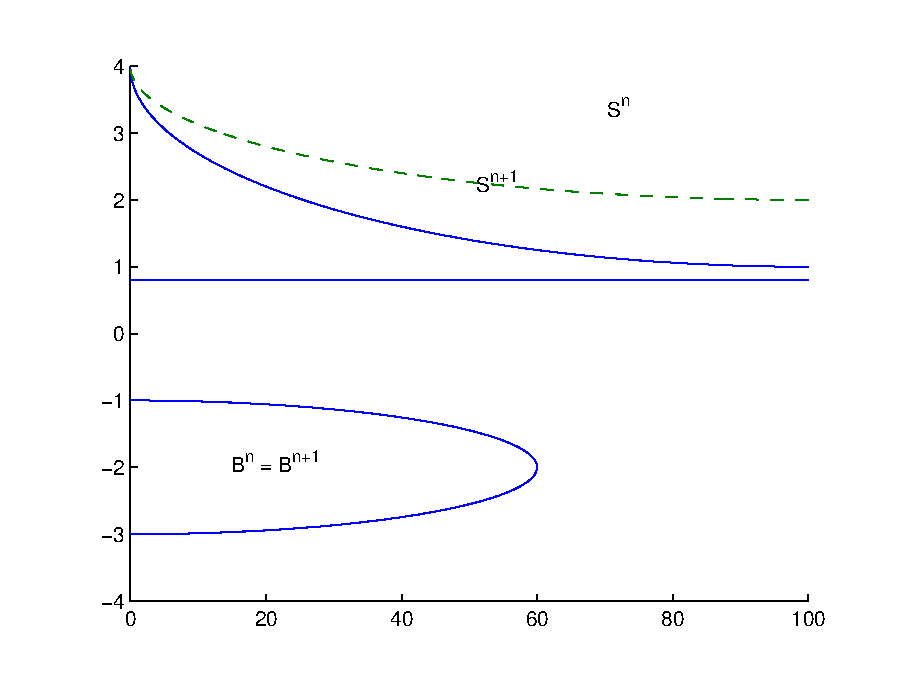
\includegraphics{SnSn+1Bn.eps}
%  \caption{Regions of $S^n$, $S^{n+1}$ and $B^n = B^{n+1}$}
%\end{figure}
%
%Define $\Delta V^{n+1}(x,q) = V^{n+1}(x,q) - V^{n}(x,q)$. According to the conditions under which the selling boundary is moved, we have 
%
%\begin{equation}\label{V}
%\begin{split}
%\Delta V_q^{n+1}(x,q) &= 0 \quad (x,q) \in S^{n}\\
%\Delta V_q^{n+1}(x,q) &> 0 \quad (x,q) \in S^{n+1}/S^{n}\\
%\LL \Delta V^{n+1}(x,q) &= 0 \quad (x,q) \in H^{n+1}\\
%\Delta V_q^{n+1}(x,q) &= 0 \quad (x,q) \in B^{n} = B^{n+1}\\
%\end{split}  
%\end{equation}
%
%\begin{figure}[hbt]\label{1ststage}
%  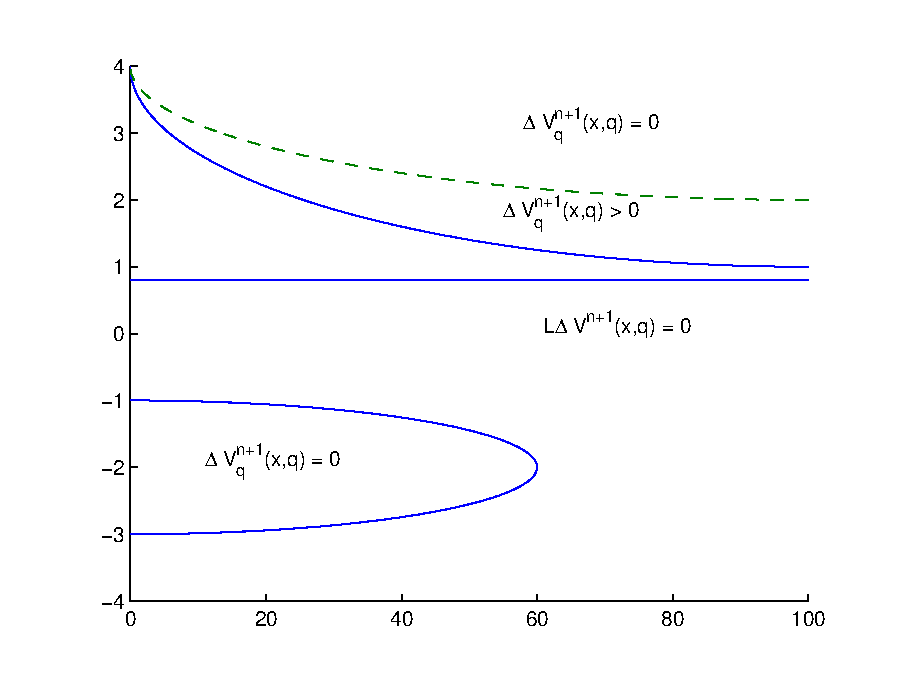
\includegraphics{deltaV.eps}
%  \caption{The equations that $\Delta V^{n+1}$ satisfies.}
%\end{figure}
%
%
%
%Since $H^{n+1}$ doesn't have isolated vertical segment except $V_1 = \{(x,0)\in H^{n+1}\}$ and $V_2 = \{(x,100)\in H^{n+1}\}$, we can take derivative with respect to $q$ to the third equation.
%
%\begin{equation}\label{Vq}
%\begin{split}
%\Delta V_q^{n+1}(x,q) &= 0 \quad (x,q) \in S^{n}\\
%\Delta V_q^{n+1}(x,q) &> 0 \quad (x,q) \in S^{n+1}/S^{n}\\
%\LL \Delta V_q^{n+1}(x,q) &= 0 \quad (x,q) \in H^{n+1}/(V_1 \cup V_2)\\
%\Delta V_q^{n+1}(x,q) &= 0 \quad (x,q) \in B^{n} = B^{n+1}\\
%\end{split}  
%\end{equation}
%
%Before moving any further, two properties of operator $\LL$ are needed. 
%
%\begin{enumerate}
%  \item It's impossible to have positive maximal interior point.
%  \item It's impossible to have negative minimum interior point.
%\end{enumerate}
%
%\begin{proof}
%Only the first one is proved, the second is the same.\\
%
%If not, there exists $x$ which is the positive maximal interior point. Then $f'(x) = 0$ and $f''(x) \leq 0$. On the other hand, $\LL f(x) = 0$. By the definition of $\LL$,
%
%\begin{equation}
%\begin{split}
%  &\frac{1}{2}\sigma^2 f'' + \kappa(\alpha - x) f' - \beta f = 0 \\
%  \Rightarrow & 0<\beta f = \frac{1}{2}\sigma^2 f'' + \kappa(\alpha - x) f' \leq 0
%\end{split}
%\end{equation}
%
%Contradiction!
%
%\end{proof}
%
%Here begins the proof of $\Delta V^{n+1}(x,0) \geq 0$.
%\begin{proof}
%
%Notice that with $q$ fixed, $f(x) = \Delta V_q^{n+1}(x,q)$ is the solution of $\LL f = 0$. Moreover, the boundary conditions are  $f(x_S)> 0$, where $(x_S,q) \in S^{n+1}/S^{n}$ and $f(x_B) = 0$, where $x_B$ is the largest $x$ satisfying $(x,q) \in B^{n} = B^{n+1}$.\\   
%
%Therefore, by the two properties of $\LL$, $f(x)$ is non-negative for all points $(x,q) \in H^{n+1}$ and it achieves its maximum at point $x_S$. By the fact that $q$ is arbitrary, 
%\begin{equation}
%  \Delta V_q^{n+1}(x,q) \geq 0 \quad (x,q) \in H^{n+1}/(V_1 \cup V_2).
%\end{equation}
%
%Together with (\ref{Vq}), 
%
%\begin{equation}\label{nonneg}
%  \Delta V_q^{n+1}(x,q) \geq 0 \quad (x,q) \in \mathbb{R}\times[0,100]/(V_1 \cup V_2).
%\end{equation}
%
%There are two cases when the selling boundary moves.
%
%\begin{enumerate}
%  \item States of $q = 0$ is isolated.
%  \item States of $q = 0$ is not isolated.
%\end{enumerate}
%
%\begin{figure}[hbt]
%  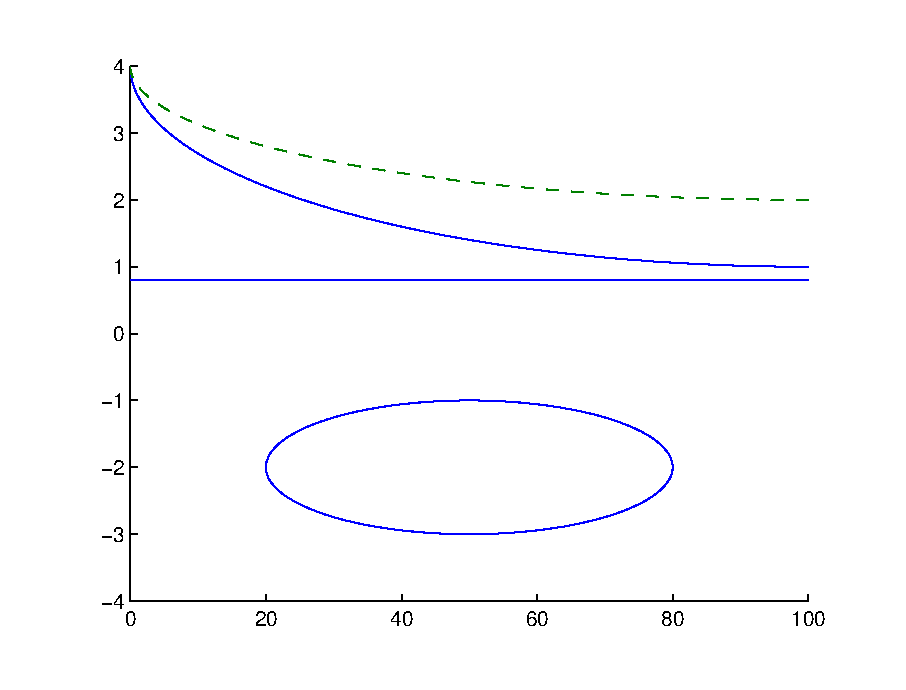
\includegraphics{Isolated.eps}
%  \caption{When states of q = 0 is isolated when selling boundary moves.}
%\end{figure}
%
%\begin{figure}[hbt]
%  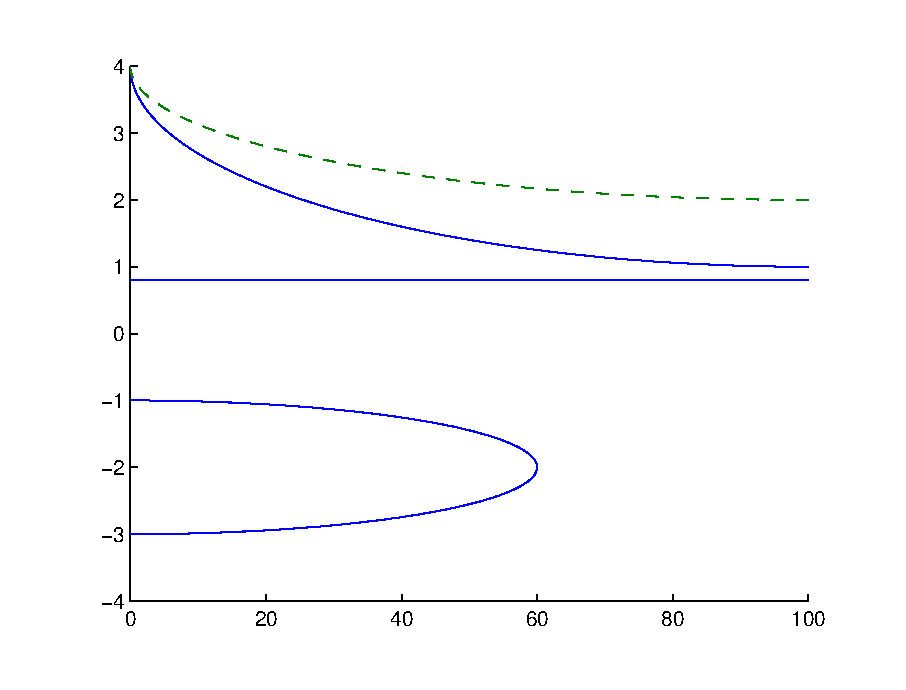
\includegraphics{NotIsolated.eps}
%  \caption{When states q = 0 is not isolated when selling boundary moves.}
%\end{figure}
%
%In the first case, $\LL \Delta V^{n+1}(x,0) = 0 \quad \forall x \in \mathbb{R}$. By the fact that both $V^{n+1}$ and $V^{n}$ are bounded, $\Delta V^{n+1}(x,0)$ is also bounded. Combine these two we have $\Delta V^{n+1}(x,0) = 0 \quad \forall x \in \mathbb{R}$. What's more, (\ref{nonneg}) shows that 
%
%\begin{equation}
%  \Delta V^{n+1}(x,q) = \Delta V^{n+1}(x,0) + \int_{0}^{q} \Delta V_q^{n+1}(x,\tau)d\tau \geq 0+0 = 0.
%\end{equation}
%
%
%In the second case, we still want to show that $\LL \Delta V^{n+1}(x,0) = 0 \quad \forall x \in \mathbb{R}$. It is trivial when $(x,0) \in H^{n+1}$. To prove the case $(x,0) \notin H^{n+1}$, another assumption is needed. \\
%
%\textbf{At a fixed level $x$, at most one of buying and selling happens which is the same as } 
%
%
%\begin{equation}
%\begin{split}
%  (x,0) \notin H^{n+1} &\Leftrightarrow \text{Buying happens at level $x$} \\
%  &\Leftrightarrow \text{(x,100) is not a selling point} \Leftrightarrow (x,100)\in H^{n+1}.
%\end{split}
%\end{equation}
%
%Because for the optimal policy, it is proved at most one of buying and selling happens and both buying strategy and selling strategy is less aggressive than the optimal one. This assumption is reasonable. In the case $(x,0) \notin H^{n+1}$,
%
%\begin{equation}\label{q100}
%    \Delta V^{n+1}(x,0) = \Delta V^{n+1}(x,100) - \int_{0}^{100} \Delta V_q^{n+1}(x,q)dq.
%\end{equation}
%
%There are only two situations for $\{(x,q)| q \in (0,100)\}$,
%
%\begin{enumerate}
%  \item $(x,q) \in B^{n+1} \Rightarrow \Delta V_q^{n+1}(x,q) = 0$  
%  \item $(x,q) \in H^{n+1} \Rightarrow \LL\Delta V_q^{n+1}(x,q) = 0$.
%\end{enumerate}
%
%Note that $f(x) = 0$ is the solution to $\LL f(x) = 0$. No matter which case, we always have $\LL\Delta V_q^{n+1}(x,q) = 0$. Use operator $\LL$ to both sides of (\ref{q100}),
%
%\begin{equation}
%\begin{split}
%    \LL \Delta V^{n+1}(x,0) &= \LL \Delta V^{n+1}(x,100) - \LL\int_{0}^{100} \Delta V_q^{n+1}(x,q)dq \\
%    &= 0 - \int_{0}^{100} \LL \Delta V_q^{n+1}(x,q)dq  = 0.
%\end{split}
%\end{equation}
%
%In sum, $\LL \Delta V^{n+1}(x,0) = 0 \quad \forall x \in \mathbb{R}$. By previous argument, $\Delta V^{n+1}(x,q) \geq 0$.
%
%\end{proof}
%

%
%
%\section{The optimal policy will sell or buy(I need to prove that it is only sell that is possible) when the price is high enough. Namely, holding region always has a higher bound.}
%
%% TODO I need to change this title.
%
% 
% 
%\section{At optimal, buy and sell won't occur at the same price level.}
%
%
%
%
%\newpage
%\section{When futures are redundant?}
%
%
%Let $F_{t,T}$ denote the price at time $t$ of future whose maturity is $T$. $Q,P$ are risk-neutral and historical measure respectively. If the prices are consistent with underlying asset price $exp(X_t)$, 
%
%\begin{equation*}
% \exp(-\beta t) F_{t,T} = E_{Q} ( \exp(-\beta T)\exp(X_T) |\mathcal{F}_t)
%\end{equation*}
%
%The discounted profit of selling one unit commodity via this future is 
%
%\begin{equation*}
%\begin{split}
%  &\exp(-\beta t) F_{t,T} - \exp(-\beta T) \int_{Q}^{Q+1}\mu(q) dq\\
%  =&  E_{Q} ( \exp(-\beta T)\exp(X_T) |\mathcal{F}_t) - \exp(-\beta T) \int_{Q}^{Q+1}\mu(q) dq\\
%  =&  E_{Q} ( \exp(-\beta T)\exp(X_T) - \exp(-\beta T) \int_{Q}^{Q+1}\mu(q) dq
%   |\mathcal{F}_t).\\
%   =&  E_{Q} ( e^{-\beta T}(e^{X_T} - \mu(Q^1_T)|\mathcal{F}_t).
%\end{split}
%\end{equation*}
%
%where $\mu(Q^1_T) = \int_{Q}^{Q+1}\mu(q) dq$. 
%
%
%Similarly total discounted cost of one unit commodity bought via this future is 
%
%\begin{equation*}
%\begin{split}
%  &\exp(-\beta t) F_{t,T} + \exp(-\beta T) \int_{Q}^{Q+1}\lambda(q) dq\\
%  =&  E_{Q} ( \exp(-\beta T)\exp(X_T) |\mathcal{F}_t) + \exp(-\beta T) \int_{Q}^{Q+1}\lambda(q) dq\\
%  =&  E_{Q} ( \exp(-\beta T)\exp(X_T) + \exp(-\beta T) \int_{Q}^{Q+1}\lambda(q) dq
%   |\mathcal{F}_t)\\
%   =&  E_{Q} ( e^{-\beta T}(e^{X_T} + \lambda(Q^2_T)|\mathcal{F}_t). 
%\end{split}
%\end{equation*}
%where $\lambda(Q^2_T) = \int_{Q}^{Q+1}\lambda(q) dq)$.
%
%
%Recall the objective function without futures.
%
%\begin{equation}
%  V(x,q) = \max_{(L,U) \in \mathcal{U}} \mathbb{E}_P \left(\int_{0}^{\infty} e^{-\beta t}(e^{X_t} - \mu(Q^1_t))dU_t - \int_{0}^{\infty}e^{-\beta t}(e^{X_t} + \lambda(Q^2_t))dL_t\right)
%\end{equation}
%
%Notice, this expectation is under historical measure. If $P = Q$, the future is redundant. If $P \neq Q$, it is not.
%
%%Assume we also have another boundary point with the same level of price on the left hand side of $(x_0,q_0)$ , i.e. $(x_0,q_1)$ where $q_1 < q_0$ and there is no other boundary point between them. Therefore
%%
%%\begin{equation*}
%%\begin{split}
%%V(x_0,q_0) &= V(x_0,q_1) + \int_{q_1}^{q_0} V_q(x_0,q) dq\\
%%&=V(x_0,q_1) + (q_1-q_0) e^{x_0} + \int_{q_1}^{q_0} \lambda(q) dq.
%%\end{split}
%%\end{equation*}
%%
%%Use operator $\LL$ to both sides, 
%%
%%\begin{equation*}
%%\LL V(x_0,q_0) = \LL V(x_0,q_1) + \LL ((q_1-q_0) e^{x_0} + \int_{q_1}^{q_0} \lambda(q) dq)
%%\end{equation*}
%%
%%By the continuity of $V_{xx}, V_{x}, V$  with respect to $q$ on the boundary, we have 
%%
%%\begin{equation*}
%%\LL V(x_0,q_0) = \LL V(x_0,q_1) = 0.
%%\end{equation*}
%%
%%So
%%\begin{equation*}
%%\LL ((q_1-q_0) e^{x_0} + \int_{q_1}^{q_0} \lambda(q) dq) = 0,
%%\end{equation*}
%%
%%which gives us
%%
%%\begin{equation*}
%%\frac{1}{2} \sigma^2 e^{x_0} + k(\alpha -x_0) e^{x_0} - \beta (e^{x_0} +\frac{1}{q_0-q_1}\int_{q_1}^{q_0}\lambda(q)dq) = 0.
%%\end{equation*}
%%
%%This can't happen if $\lambda(q)$ is strictly increasing on $[q_1,q_0]$, because by (\ref{geq})
%%
%%\begin{equation*}
%%\begin{split}
%%\frac{1}{2} \sigma^2 e^{x_0} + k(\alpha -x_0) e^{x_0} - \beta e^{x_0} \geq \beta \lambda(q_0) >\frac{1}{q_0-q_1}\int_{q_1}^{q_0}\lambda(q)dq .
%%\end{split}
%%\end{equation*}
%%
%%Assume that there is another boundary point $(x_0,q_2)$ at the right hand side of $(x_0,q_0)$, namely $q_2>q_0$ and the region between them are holding region. By the previous result, there can't be a boundary point on the right hand side of $(x_0,q_2)$. Let $(x_0,q_3)$ where $q_3 > q_2$, then $(x_0,q_3)$ must belong to injection region.
%%
%%Similarly
%%
%%\begin{equation*}
%%\begin{split}
%%\LL V(x_0,q_2) &= 0 \\
%%\LL V(x_0,q_3)& < 0\\
%%V(x_0,q_3) &= V(x_0,q_2) + (q_3-q_2) e^{x_0} + \int_{q_2}^{q_3} \lambda(q) dq.
%%\end{split}
%%\end{equation*}
%% 
%%Use operator $\LL$ to both sides of the last equality and use the top two 
%%
%%\begin{equation*}
%%0>\LL V(x_0,q_3) = 0 + (q_3-q_2) (\frac{1}{2} \sigma^2 e^{x_0} + k(\alpha -x_0) e^{x_0} - \beta (e^{x_0} +\frac{1}{q_3-q_2}\int_{q_2}^{q_3}\lambda(q)dq)).
%%\end{equation*}
%%
%%This shows that 
%%
%%\begin{equation*}
%% \frac{1}{2} \sigma^2 e^{x_0} + k(\alpha -x_0) e^{x_0} - \beta (e^{x_0} +\frac{1}{q_3-q_2}\int_{q_2}^{q_3}\lambda(q)dq) < 0.
%%\end{equation*}
%%
%%Let $q_3 \rightarrow q_2$, 
%%
%%\begin{equation*}
%% \frac{1}{2} \sigma^2 e^{x_0} + k(\alpha -x_0) e^{x_0} - \beta (e^{x_0} +\lambda(q_2) )\leq 0.
%%\end{equation*}
%%
%%On the other hand, $(x_0,q_2)$ is the boundary point, thus
%%
%%\begin{equation*}
%% \frac{1}{2} \sigma^2 e^{x_0} + k(\alpha -x_0) e^{x_0} - \beta (e^{x_0} +\lambda(q_2) )\geq 0.
%%\end{equation*}
%%
%%Combine those two,
%%
%%\begin{equation*}
%%\frac{1}{2} \sigma^2 e^{x_0} + k(\alpha -x_0) e^{x_0} - \beta (e^{x_0} +\lambda(q_2) )= 0.
%%\end{equation*}
%%
%%
%
%
%
% 
% %%%%%%% This part is wrong %%%%%%%%%%%%
%% \section{Withdraw region}
%% In this section we would like to show that if $(M, \q)$ is a withdrawing point and $M$ is big enough, any point $(x,\q)$ where $x>M$ is also a withdrawing point. If not, let $(x_3,\q)$ be the point changes from withdrawal to holding. The smooth fit conditions tell us
%% \begin{equation*}
%% h(x_3) = 0 \quad h'(x_3) =0
%% \end{equation*}
%% where $h(x)$ is defined in the previous section. Define
%% \begin{equation*}
%% x_4 = \inf\{x>x_3|h'(x)=0\}.
%% \end{equation*}
%%If $x_4 < +\infty$, 
%%\begin{equation*}
%%h'(x_4) =0 \quad h''(x_4) \leq 0 .
%%\end{equation*}
%%However, it is impossible to have (\ref{hPDE}) hold at point $x_4$ when $x_4$ is big enough. Thus $x_4 = +\infty$ namely $h'(x) > 0~ \forall x > x_3$. On the other hand, previous section tells us there must be another withdrawing point $x_5 > x_3$. Still by smooth fit conditions at $x_5$, $h'(x_5) = 0$. Contradiction! \\
%%
%%Actually it is possible to quantify 'big enough' in this section. $x^*$ is big enough if expression $
%%- \frac{1}{2}\sigma^2 e^x + k (x- \alpha)e^x + \beta(e^x - \mu)$ is positive when $x\geq x^*$.
%%I want to show that it is impossible to inject when the price is big enough. And amazingly I should that it is impossible to change from holding to injection. First recall the PDE we have.
%%\begin{equation}
%%\frac{1}{2}\sigma^2f''(x) + k(\alpha-x)f'(x) - \beta f(x) = - \frac{1}{2}\sigma^2 e^x + k(x-\alpha)e^x + \beta(e^x - \mu) 
%%\end{equation}
%%At the injection point $x_0$, we have $f(x_0) = \mu + \lambda$ and $f'(x_0) = 0$. If we approach $x_0$ from holding region we should have\footnote{$f''$ is not continuous at point $x_0$.}
%%\begin{equation}
%%\frac{1}{2}\sigma^2f''(x_0) - \beta (\mu+\lambda)= - \frac{1}{2}\sigma^2 e^{x_0} + k(x_0-\alpha)e^{x_0} + \beta(e^{x_0} - \mu) 
%%\end{equation}
%%Therefore,
%%\begin{equation}
%%\frac{1}{2}\sigma^2f''(x_0)= - \frac{1}{2}\sigma^2 e^{x_0} + k(x_0-\alpha)e^{x_0} + \beta(e^{x_0} + \lambda)
%%\end{equation}
%%Let 
%%\begin{equation}
%%t(x) =  - \frac{1}{2}\sigma^2 e^{x} + k(x-\alpha)e^{x} + \beta(e^{x} + \lambda)
%%\end{equation}
%%If  $t(x_0) > 0$ then $f''(x_0) > 0$. However, $f$ has the maximum value as $\mu + \lambda$ and $f'(x_0) = 0$, therefore $f''(x_0) \leq0$. Contradiction. Therefore, we must have $t(x_0) \leq 0$.  Then $f(x) = \mu + \lambda~for ~\{x>x_0\}\cap\{injection~region\} $. If we approach $x_0$ from above we should have 
%%\begin{equation}
%%\frac{1}{2}\sigma^2f''(x_0) + k(\alpha-x_0)f'(x_0) - \beta f(x_0) < - \frac{1}{2}\sigma^2 e^{x_0} + k(x_0-\alpha)e^{x_0} + \beta(e^{x_0} - \mu)
%%\end{equation}
%%\begin{equation}
%%- \beta (\mu+\lambda) < - \frac{1}{2}\sigma^2 e^{x_0} + k(x_0-\alpha)e^{x_0} + \beta(e^{x_0} - \mu)
%%\end{equation}
%%\begin{equation}
%%0 < - \frac{1}{2}\sigma^2 e^{x_0} + k(x_0-\alpha)e^{x_0} + \beta(e^{x_0} + \lambda) = t(x_0)
%%\end{equation}
%%Contradiction!
%%
%%Next I want to show when the price is low enough we always inject!
%%It is easy to show that it is impossible to withdraw when the price is low enough since the \limits PDE left = 0 ,right < 0 which contradicts the definition of withdraw region.
%% 
%%
%%\section*{Conclusion}
%%
%%\bibliographystyle{unsrt}
%%
%%\bibliography{sample}
%%
%%----------------------------------------------------------------------------------------
%%
\end{document}